\subsection{Benchmarking} %Correlating Microarchitecture with Performance\jled{change to ``Benchmarking''?}}
\label{sec:benchmark}


To explore NVIDIA Kepler architecture, we create microbenchmarks tailored for each characteristic.
% Our following observations are drawn from analyzing the execution time of the microbenchmarks.
The kernel code is written in assembly and compiled into {\tt cubin} by our assembler, and then called by CUDA APIs.
The instructions inside assembly loop are abundant to cover branch overhead without exceeding L1 instruction cache.
%All assembly kernel codes are designed small enough to fit into the L1 instruction cache.
For timing accuracy, the same CUDA kernel code is tested for hundreds of times, and the average is used for our analysis.
Timing ticks are recorded by {\tt S2R R0, SR\_CLOCKLO} instruction, in which {\tt S2R} is special register to general
purpose register and  {\tt SR\_CLOCKLO} is the clock register. Then time is calculated and written to global memory.
%We run each benchmark program twice, disregarding the first run to avoid compulsory instruction cache misses.
Two metrics are benchmarked: latency and throughput. Latency is tested by a succession of dependented instructions by
launching a block of $32$ threads. Throughput is tested by a succession of independent instructions by launching enough
threads(e.g. $26$ blocks, each block with $512$ threads for Kepler) to make full use of CUDA cores and bandwidth.
%We use similar testing method with Fog's in~\cite{fog}.

As shown in~\ref{fig:workflow}, we tune the assembly codes of our microbenchmarks using our assembler.
From the tuning process, we correlate microarchitecture characteristics with the benchmark performance, which is useful
to optimize program snippets in real applications.
% According to the performance tuning results, we
The correlation is presented as meaningful observations, which are categorized into four microarchitectural features:  {\tt register} bank, {\tt
control} code,  {\tt arithmetic} throughput, and {\tt memory} operation.


\begin{figure*}
    \begin{subfigure}[htbp]{0.3\textwidth}
        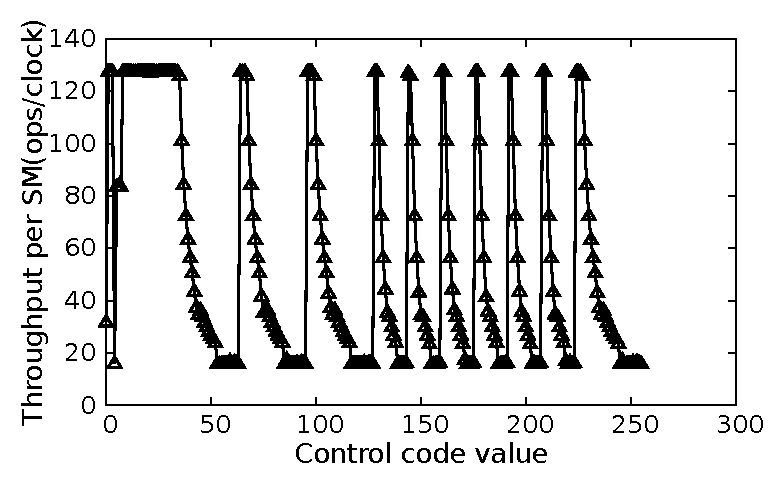
\includegraphics[width=2.1in]{ctrl}
        %\subcaption{Control code regulates {\tt FFMA} throughput.} %\jled{8-bit control code value} \jled{ops/cycle? or IPC?}}
        \subcaption{}
        \label{fig:control_throughput}
    \end{subfigure}
    \begin{subfigure}[htbp]{0.3\textwidth}
        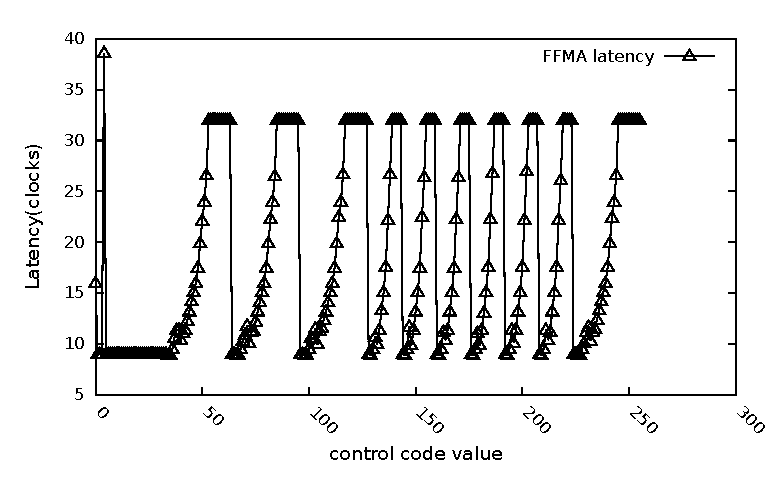
\includegraphics[width=2.1in]{ctrl_latency}
        \subcaption{}
        %\subcaption{Control code regulates {\tt FFMA} latency.} %\jled{8-bit control code value}}
        \label{fig:control_latency}
    \end{subfigure}
    \begin{subfigure}[htbp]{0.3\textwidth}
        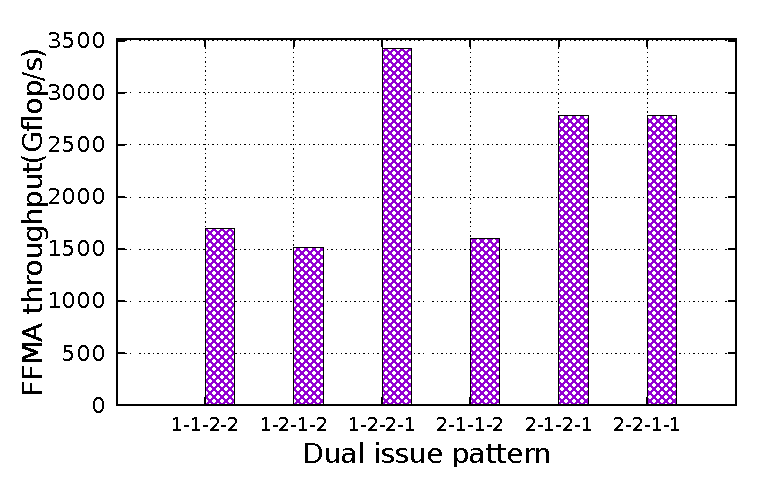
\includegraphics[width=2.1in]{pattern}
        \subcaption{}
        %\subcaption{Peak {\tt FFMA} throughput(1: single issue, 2: dual issue).}%\jled{Y-axis is performance?}}
        \label{fig:control_pattern}
    \end{subfigure}
    \caption{Different control code impact on performance(subfigure(\subref{fig:control_pattern}), 1$\rightarrow$single
    issue, 2$\rightarrow$dual issue).}
    \label{fig:control_code}
\end{figure*}


{\em {\bf Observation 1--[Register Bank]}:
Source registers may cause register bank conflicts that degrade instruction throughput.}
\begin{table}[htbp]
    \caption{The efficiency of instruction throughput varies with difference register bank distribution. {\it Inst} :
instruction pattern, {\it Th/SM}: the instruction throughput per SM, {\it Eff}: efficiency of throughput, {\tt Conf}: register bank conflicts.}
\centering
\scalebox{0.9} {
\begin{tabular}{|c|c|c|c|}
\hline
Inst &Th/SM&Eff&Conf\\
\hline
{\tt FFMA R5,R4,R1,R0}&127.50&66.40\%&0\\
\hline
{\tt FFMA R2,R4,R1,R0}&127.50&66.40\%&0\\
\hline
{\tt FFMA R5,R2,R1,R0}&119.18&62.07\%&2-way\\
\hline
{\tt FFMA R3,R2,R1,R0}&119.18&62.07\%&2-way\\
\hline
{\tt FFMA R5,R9,R3,R1}&94.52&49.23\%&3-way\\
\hline
{\tt FFMA R11,R9,R3,R1}&94.52&49.23\%&3-way\\
\hline
{\tt FMUL R4,R1,R0}&127.50&66.40\%&0\\
\hline
{\tt FMUL R4,R2,R0}&119.17&62.06\%&2-way\\
\hline
\end{tabular}
}
\label{tab:th}
\end{table}


\begin{table}[htbp]
\caption{Register bank distribution.}
\centering
\scalebox{0.9} {
\begin{tabular}{|c|c|c|c|c|c|c|c|c|}
\hline
    {\tt Bank0}&{\tt R0}&{\tt R2}&{\tt R8}&{\tt R10}&{\tt R16}&{\tt R18}&{\tt R24}&{\tt R26}\\
\hline
    {\tt Bank1}&{\tt R1}&{\tt R3}&{\tt R9}&{\tt R11}&{\tt R17}&{\tt R19}&{\tt R25}&{\tt R27} \\
\hline
    {\tt Bank2}&{\tt R4}&{\tt R6}&{\tt R12}&{\tt R14}&{\tt R20}&{\tt R22}&{\tt R28}&{\tt R30}\\
\hline
    {\tt Bank3}&{\tt R5}&{\tt R7}&{\tt R13}&{\tt R15}&{\tt R21}&{\tt R23}&{\tt R29}&{\tt R31}\\
\hline
\end{tabular}
}
\label{tab:reg}
\end{table}


Shared memory bank conflict is well-known as an important performance factor for CUDA programming.
Recent research~\cite{lai} noticed that register bank conflict is also nontrivial to performance.
To probe register bank distribution on Kepler, our microbenchmark measures instruction throughput for different combinations of {\tt FFMA}
register operands.
Table~\ref{tab:th} shows one example combination resulting in various efficiency numbers.
The rightmost column represents the number of register bank conflicts recorded from our experiments.
This experiment is conducted in single issue mode by setting control code to 0x20.
Theoretically, without dual issue, the peak efficiency is $(4\times32)/192=128/192=66.67\%$, in which $4$ is the number of warp schedulers and $32$
is the number of threads in a warp.
In fact, we observe that both single- and dual-issue mode produce the same throughput behavior for bank conflicts.
 % variance of instruction throughput.
From our experiments on Kepler architecture, we observe:
\begin{itemize}
\item The destination register will not contribute to bank conflict, no matter which bank is assigned to it.
\item When source registers have 2-way or 3-way register bank conflicts, the throughput of float instructions will drop by 2.33\% and 17.17\% respectively in single issue mode.
\item Our microbenchmark finds out a proper distribution of registers to eliminate bank conflict.
     Table~\ref{tab:reg} lists registers and their corresponding banks, which is consistent with GTX680~\cite{lai}, though 
        K20 is different from GTX680 in maximal registers per thread and instruction encoding.
        %\\
% bank0$\Leftarrow$($Ridx \% 8 < 4$ \&\& $Ridx \% 2 == 0$) \\
% bank2$\Leftarrow$($Ridx \% 8 < 4$ \&\& $Ridx \% 2 == 1$) \\
%bank1$\Leftarrow$($Ridx \% 8 > 4$ \&\& $Ridx \%2 == 0$) \\
%bank3$\Leftarrow$($Ridx \% 8 < 4$ \&\& $Ridx\% 2 == 1$)\\
%where $Ridx$ is the register number.
%This rule will guide the performance tuning of SGEMM code.

\end{itemize}


{\em {\bf Observation 2--[Control Code]}:
Warp scheduling and issue mode are tunable by modifying control codes which regulate instruction issue.}

Starting with the Kepler architecture, NVIDIA has been moving some control logics off the chip and into kernel
instructions which are determined by the assembler~\cite{lai,maxas}. This evolution provides programmers the opportunity to
make globally optimal scheduling decisions and other control optimizations if an assembler is available. The disassembly
code from sample programs and cuBLAS library indicates that every $64$-bit control binary code controls $7$ instructions
exactly as Figure~\ref{fig:assemblycode} shows.
% a control code is placed before $7$ instructions, and it
We identify that both the highest $6$ bits and the lowest
$2$ bits are the {\em opcode} of the scheduling instruction, and the middle $56$ bits are used to control the execution of $7$
instructions, each of which is assigned to $8-bit$ control code.

We figure out control code meanings by statically examining the disassembly codes of cuBLAS and
dynamically benchmarking instruction sequence of different control codes.
In this way, we discover that bit-$4$ represents shared memory dependency barrier, bit-$5$ represents global memory dependency
barrier, and bit-$7$ indicates a texture cache dependency barrier due to its weak consistency cache model.
Unexpected values will be loaded if the bit-$7$ is not set.
%\jled{Wrong bit number, bit-4 not 4th bit! What about bit-$6$?? Please check the correctness.}
% We verify the $7$\textsuperscript{th} bit of the control
% code of {\tt TEXDEPBAR} instruction is set to $1$, to
% indicate a texture dependency barrier of texture cache due to its weak consistent memory model.
We use the latency of {\tt FFMA} instruction to crack $0-3$ bits of its control code.
Figure~\ref{fig:control_code}(\subref{fig:control_throughput}) and
Figure~\ref{fig:control_code}(\subref{fig:control_latency}) show {\tt FFMA}'s throughput and latency when its control
code varies from $0$ to $255$.
% Thus, most throughputs achieve the maximum when the control code's value is smaller than {\tt 0x20} because of no set suspension.
% Obvious periodicity is shown with size $16$ after the control code's value reaches {\tt 0x20}.
After 0x20, both the throughput and latency show obvious periodicity.
For each period, by increasing the value of bits $0-3$, the throughput of {\tt FFMA} drops and its latency raises by different rates. 
%\jled{the period size is different! why?}
This phenomenon implies that the four lower bits stores the number of stall cycles before issuing
an instruction.
Our microbenchmarking reveals some specific patterns of control codes:
% Furthermore, the microbenchmarking reveals some specific patterns of control codes:

\begin{itemize}
\item When the control code is set to 0x00, the scheduler suspends a warp of the instructions for $16$ cycles.
\item 0x2n means a warp is suspended for $n$ cycles before issuing the next instruction, where $n=0, 1,\dots, 15$.
\item 0x20 means single issue mode, while 0x04 means dual-issue mode.
While two consecutive instructions are controlled by 0x04 and 0x05 respectively, the throughput could reach the maximum.
        %\jled{relation with Figure?}
\end{itemize}

{\em {\bf Observation 3--[Arithmetic Throughput]}:
With a proper control code pattern and register allocation, {\tt FFMA}
instruction throughput can approach the theoretical peak in dual issue mode.}

It's very intricate to tune instruction execution to improve instruction throughput. The previous work~\cite{lai}
reports the maximal throughput of {\tt FFMA} per SM as $132$, which is only $68.75\%$ efficiency of the theoretical
throughput. Our microbenchmark reveals several key points of tuning {\tt FFMA} throughput to $97\%$ efficiency.
First, the control code must be set properly to dual issue adjacent instructions. 
Second, the ratio and interval of dual issue {\tt FFMA} instructions must be tuned into a specific pattern.
Third, the first instruction of the core loop needs to be aligned. This restriction is
caused by the aligned position of control code in the instruction sequence.
Last, each {\tt FFMA} requires three source registers, thus in dual issue, two {\tt FFMA} requires six source registers, but
Kepler only provides four register banks.
Instruction order must be adjusted to use Kepler's operand collector mechanism~\cite{collector,tarjan2012policy} to avoid register bank conflicts. 

%Figure~\ref{fig:warp} illustrates {\tt FFMA} dual issuing. There are $32\times 6=192$ cores on
Figure~\ref{fig:warp} illustrates the mapping of {\tt FFMA} instructions to cores in dual issue mode on one SM. There are $32\times 6=192$ cores on
one SM, the middle $32$ cores are shared by two warp schedulers, and four warp schedulers are available per SM. 
In single mode, each warp scheduler issues instruction to $32$ cores, which
yields $4\times32/192=66.67\%$efficiency. 
In dual issue mode, two warp schedulers must use the shared cores alternately to avoid resource conflicts.
The jagged green and red blocks show a proper phase shift between two warp's executing pace so that they could get
access to the shared computing unit in turn.
The optimal ratio of dual issue to single issue is $2:2$ theoretically, 
\( \begin{pmatrix} 4 \\ 2 \end{pmatrix} \) $=6$ combinations for mixed single and dual issue
pattern inside a $7$ instructions scheduling block (Figure~\ref{fig:control_code}(\subref{fig:control_pattern})).
We choose the best {\tt 1-2-2-1} pattern in our SGEMM implementation.
As shown in Table~\ref{tab:ffma}, these optimizations together improve {\tt FFMA}'s throughput to $190$ ops/clock
, which is very close to the theoretical peak $192$ ops/clock.
%Since each SM of extra computing unit is shared among two warps, when all threads are trying to fully dual issue every
%two adjacent {\tt FFMA}s, half of the scheduler would stall due to computing resource conflict.
\begin{figure}[htbp]
\begin{center}
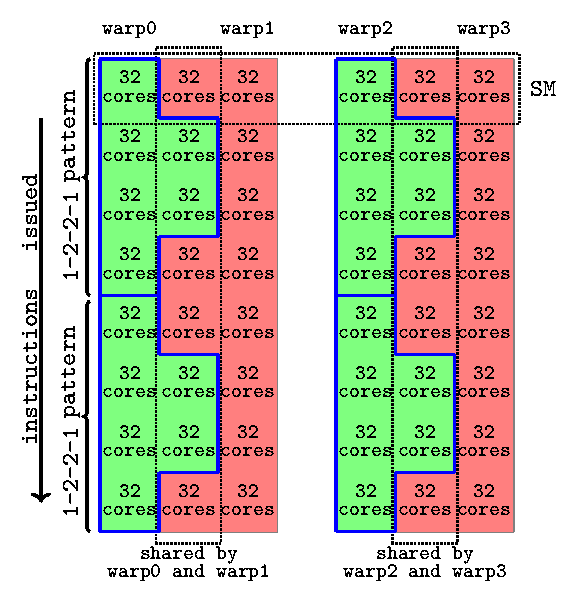
\includegraphics[scale=0.65]{warp}
    \caption{An illustration of dual issue to achieve peak throughput}
\label{fig:warp}
\end{center}
\end{figure}

\begin{table}[htbp]
\caption{Floating-point instruction throughput on Kepler}
\centering
\scalebox{0.9} {
\begin{tabular}{|c|c|c|c|}
\hline
Inst &operation&single issue&dual issue\\
\hline
{\tt FFMA} &c=a*b+c&127.52&190.35 \\
\hline
{\tt FMUL} &c=a*b&127.52&190.35 \\
\hline
{\tt FADD} &c=a+b&127.52&191.50\\
\hline
\end{tabular}
}
\label{tab:ffma}
\end{table}

{\em {\bf Observation 4--[Memory]}: For higher memory bandwidth, shared memory prefers the $64-bit$ load
instruction {\tt LDS.64} while global memory prefers the load instruction with texture cache {\tt LDG}.}

For GPU memory hierarchy we focus on the programmer-controllable memory resources, shared memory, and global memory.
On NVIDIA GPU architecture, there are different memory access widths (32-bit, 64-bit, 128-bit) and paths (through L2
cache or texture cache).
In fact, both NVIDIA documents and previous studies~\cite{tan} pointed out that wider
instructions have longer pipeline latency.
Our benchmarking confirms this phenomenon and also identifies several bandwidth issues for memory optimization.

Intuitively, a wider load operation should achieve higher bandwidth.
We test the bandwidth of shared memory instructions with different widths, i.e. {\tt LDS.32}, {\tt LDS.64},
and {\tt LDS.128}.
The instructions are arranged to avoid shared memory bank conflict.
% In this experiment, the amount of data are projected to the number of load instructions.
%Assume the data can be loaded by $4N$ {\tt LDS.32} instructions,
%then $2N$ {\tt LDS.64} or $4N$ {\tt LDS.32} instructions are needed.
Figure~\ref{fig:lds_bw} compares the sequential memory access bandwidth of the three instructions by increasing the data volume.
{\tt LDS.64} achieves the highest bandwidth $137GB/s$, which is about $76\%$ of the peak bandwidth\footnote{The
theoretical shared memory bandwidth for each SM can be calculated as $Bandwidth = f_{core} \times Width \times Warpsize$ in
bytes, where $f_{core}$ is the frequency of a CUDA core, $Width$ is bank width, $Warpsize$ is warp size.}.

% global memory
Two paths are used to load data from global memory, through L2 cache by {\tt
LD} instruction or texture cache by {\tt LDG} instruction.
We launch $26$ thread blocks each with $512$ threads, and specify that each thread accesses four words in a stride of $4 \times blockDim.x \times gridDim.x$.
The total global memory accessed is $256$MB.
We benchmark that each {\tt LDG.128} achieves $131$GB/s, while {\tt LD.128} only achieves $76$GB/s.
%Our benchmark confirms that {\tt LDG} achieves higher bandwidth than {\tt LD}.
% , which has been identified by previous work~\cite{tan}.

\begin{figure}[htbp]
\begin{center}
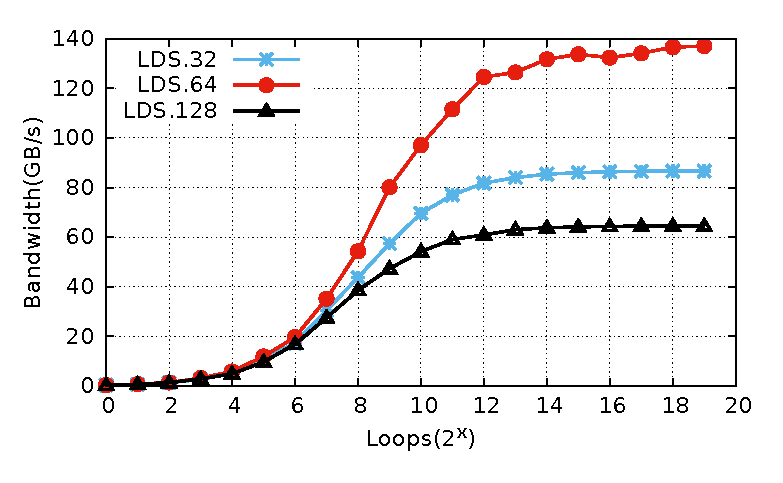
\includegraphics[scale=0.5]{lds_bandwidth}
    \caption{ Bandwidth of {\tt LDS.32}, {\tt LDS.64} and {\tt LDS.128}}
\label{fig:lds_bw}
\end{center}
\end{figure}
